\documentclass[a4paper,10pt,twocolumn]{jsarticle}
\pagestyle{empty}	
\usepackage[top=15truemm,bottom=15truemm,left=25truemm,right=25truemm]{geometry}
\usepackage[haranoaji]{pxchfon}
\usepackage[deluxe]{otf}
% 数式
\usepackage{amsmath,amsfonts}
\usepackage{bm}
% 画像
\usepackage[dvipdfmx]{graphicx}

\usepackage{here}
\usepackage{titlesec}

\setboldgothicfont[0]{HaranoAjiGothic-Heavy.otf}% 原ノ味ゴシックHeavy

\titleformat*{\section}{\large\bfseries\gtfamily}
\titleformat*{\subsection}{\normalsize\bfseries\gtfamily}

\begin{document}

\title{\textbf{\textsf{利き手を変えてスポーツをする}}}
\author{\textbf{ME2208 \textsf{\CID{8705}橋 尚太郎}}}
\date{}
\maketitle
\section{はじめに}
私は、生まれつき右利きだが、左利きでスポーツをすることがある。
その理由は、練習をして左利きに転向したからだ。私は、柔道と野球とハンドボールを左利きで行う。
そこで、本発表ではスポーツの利き手を転向した経験から、私自身が感じたこと、考えたこと、興味があって調べたことを述べる。
具体的な内容は、"利き手を転向して良かった" と感じたスポーツの選出と、利き手の転向に関する調査である。
\section{発表の概要}
\begin{itemize}
    \item 利き手を転向した理由
    \item 利き手を転向して良かったスポーツ
    \item 利き手の転向方法
    \item 結論
\end{itemize}
\section{利き手を転向した理由}
利き手の転向は、それぞれ時期が異なり、順番がある。転向した順番に経緯を説明する。
\vspace{3mm}
\subsection{柔道}
私は、柔道を始めてすぐ(小2頃)に、先生の勧めで左利きに転向した。先生が転向を勧めた意図は、
引き手(相手の袖を持つ手)を利き手の右手にすることで、組み手を有利にするためだったと推測される。
\vspace{3mm}
\subsection{野球}
私は、野球を習い始める前(小3頃)に、親の勧めで左利きに転向した。理由は2つあり、1つ目は親が誤って左投げ用のグラブを購入したことだ。
2つ目は、私が左手でもボールを投げているのを見て、野球で左投げは有利になるから勧めてくれたそうだ。
打撃は、左右を転向してもしなくても良かったが、左投右打は野球で不利であるため左打ちにした。
\vspace{3mm}
\subsection{ハンドボール}
高専1年次に始めたハンドボールは、野球の投げ方が参考になったため、既に転向している左投げですることにした。
\section{転向して良かったスポーツ}
\subsection{柔道}
柔道をするにあたって、利き手を転向することで、組み手は改善された。さらに、元来の右の技も掛けられるため、左右の技を使えるようになった。
柔道の競技中は、使う技の利き手は自由である。そのため、左右のどちらの技を相手に掛けるかは戦略にすることができる。
柔道の戦略のイメージをを図\ref{judo}に示す。
\begin{figure}[h]
    \centering
    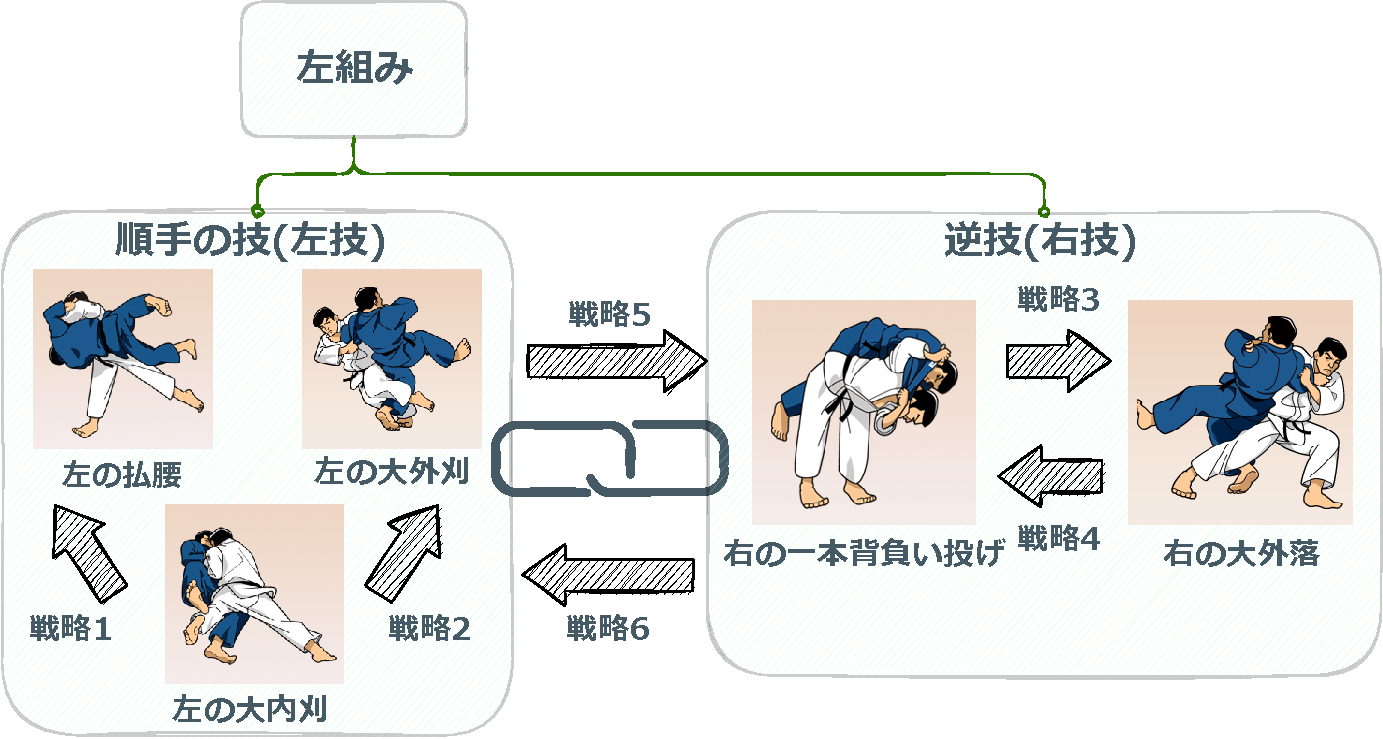
\includegraphics[scale=0.34]{img/judo.pdf}
    \caption{柔道の戦略のイメージ\cite{judo}}
    \label{judo}
\end{figure}

\subsection{野球とハンドボールについて}
野球において、利き手を転向したことによる恩恵は、柔道と比べて少ない。
打撃の面では転向前よりもバットコントロールがしやすくなった。守備に関しては、ポジションが外野であったため、
転向前と比べて有利になったことはない。野球は、役割が分担されている団体競技のため、個人のパフォーマンス向上よりもチームで連携することが戦略になる。つまり、個人が利き手を変えることは、戦略として意味が薄いと考えられる。
ただし、スイッチヒッターは例外だ。ハンドボールにおいては、メリットどころかデメリットが挙げられた。それは、サイドポジションからのシュートが打ちにくいことだ。

\section{方法}
この章では、利き手を変えてスポーツをする方法について解説する。また、イメージトレーニングの概要を図\ref{training}に示す。
\vspace{3mm}
\subsection{イメージ通りに体を動かす}
利き手を変える直感的な方法は、元の利き手の動きを反対側で真似ることだ。
それは、利き手と反対の手を左右対称に動かすことを意味する。この行動で大切なことは、
利き手と反対を使うときのイメージを明確にすることだ。\cite{takei_sou}私は、
この方法を柔道と野球で試した。柔道と、野球の打撃は上手くできたが、野球の投球動作が上手くできなかった。
そこで、利き手を変更する方法ではなく、利き手に応じた体の使い方に着目して調査を行った。
\vspace{3mm}
\subsection{人体は左右対称ではない}
人体は脳の命令によって制御される。脳は右脳と左脳があり、右脳が左半身、左脳が右半身を制御する仕組みになっている。
よって、右利きの動作は、左脳の働きが起因する。逆に左利きの動作は右脳の働きが起因する。
また、右脳と左脳は、それぞれ思考の役割が異なる。左脳が論理的思考を、右脳が直感的思考を司る。
つまり、利き手を変えることは、思考の役割が異なる脳を使って身体を動かすことだ。
すなわち、普段から使っていない脳を使うため、一般的には困難であることが分かる。
さらに、人体は構造上左右非対称である。なぜなら、内蔵の位置が左右非対称であるからだ。
そのため、総合的な人間の重心の位置は左右非対称となり、バランスの取り方が左右で異なる。\cite{balance}
利き手を変えるためには、これらの非対称性を考慮したトレーニングにより、体を思い通りにコントロールできると考えられる。
\vspace{3mm}
\subsection{脳を使う}
スポーツをする時には、イメージトレーニングをすることがある。イメージトレーニングは、実際には動かず“頭の中で”体を動かすイメージを行うことである。\cite{img_training}
図\ref{training}にイメージトレーニングの概要を示す。
これを利き手を変えることに応用する。つまり、利き手が逆の人の動きを観察し、それを見ながらイメージを作り、自分の動きを重ね合わせる。
これだけでは、左右対称の動きになるので、利き手に応じて体の重心移動のさせ方を調整する。これらで形を作ることができたので、
力加減を調整する。
\vspace{3mm}
\subsection{バランスを取る}
ここでは、野球の制球難を改善するための利き手に応じたバランスの取り方(重心移動のさせ方)について解説する。\cite{balance}
\begin{itemize}
    \item 右の場合、直線運動で(ストレートパンチを打つイメージで)重心を真っ直ぐ移動させる。
    \item 左の場合、回転運動で(フックパンチを打つイメージで)重心を回転させながら移動させる。これは、左利き独特の体の回転を活かしたボールや打撃や技に繋がる。
\end{itemize}

\begin{figure}[H]
    \centering
    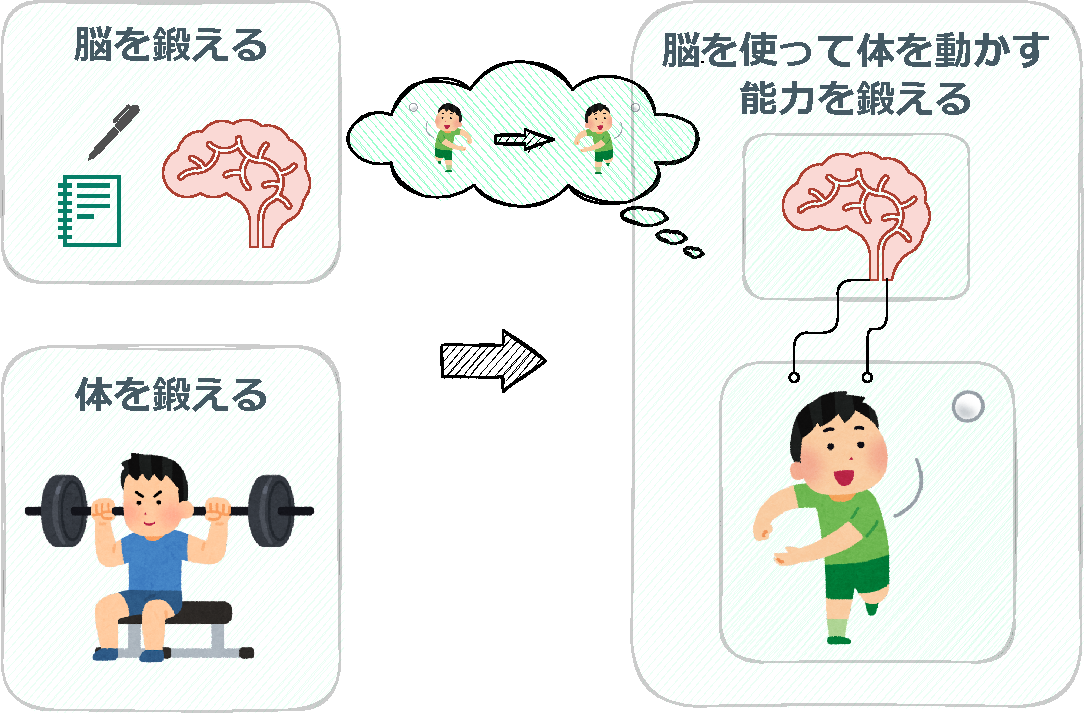
\includegraphics[scale=0.36]{img/training.pdf}
    \caption{イメージトレーニングの概要}
    \label{training}
\end{figure}

\section{まとめ}
本発表では、私が利き手を変えてスポーツをした経験から体感したことや、感じたことについて報告した。
利き手を変えることで、有利になったり、競技をしやすくなったスポーツと、逆に競技がやりにくくなったスポーツがあることが明らかになった。
また、利き手を変えることに苦労した体験から方法を調査した。その結果、利き手の転向は、動きのイメージだけではなく、人体の非対称性に考慮した、体の動かし方が重要であることが明らかになった。
利き手が違うと、便利に感じたり、そうでないときもあるが、利き手を意識するときには、"利き手は個性である" ということを心に止めて頂きたい。

\begin{thebibliography}{4}
    \bibitem[1]{judo}【柔道チャンネル】柔道技解説. \\ https://www.judo-ch.jp/dictionary/\\technique/ (参照 2022年6月20日).
    \bibitem[2]{takei_sou}武井壮の両利き理論. \\ https://www.youtube.com/watch?v=YluJhW0FYcM (参照: 2022年6月20日).
    \bibitem[3]{balance}野球専門・動作解析サポート BASEBALL ONE, 右ピッチャーと左ピッチャーは投げ方が違う?!\\ https://www.youtube.com/watch?v=0v18Nh0CCC0. (参照: 2022年6月20日).
    \bibitem[4]{img_training}【緊張をほぐす方法】プロアスリートから学ぶ『イメージトレーニング』のやり方 | ビジネス×スポーツ『MELOS』, MELOS(メロス). https://melos.media/business/39535/ \\ (参照 2022年6月20日).
\end{thebibliography}

\end{document}